%\mychapter{4}{Dimensionality Reduction}

\subsection{Dimensionality reduction}\label{spectral decomp}
In this section, we review some linear and non-linear dimensionality reduction techniques. We focus on spectral dimensionality reduction methods where the low dimensional model is obtained from spectral decomposition of an $n \times n$ positive semidefinite (PSD) proximity matrix (see appendices \ref{SVD} and \ref{proximity}). We start by defining dimensionality reduction and outlining steps of spectral dimensionality reduction. Next, we give a brief description of PCA and the diffusion maps algorithm for dimensionality reduction. In later sections, we compare the performance of PCA and diffusion maps on our spike train data set.


\subsubsection{Overview of spectral dimensionality reduction}
Let $\textbf{X} = \displaystyle \{\vect{x}_{1}, \ldots , \vect{x}_{n} \}$ be a set of $n$ data points, each of which is associated with $N$ features, so that each $\vect{x}_{i}$ is a point in a high dimensional space $\R^{N}$. For convenience, we often view the set of data points $\Bm{X}$ as a matrix, $\Bm{X} \in \mathbb{R}^{n \times N}$. Assume that the data points lie on or near an underlying $l$-dimensional manifold embedded in the high dimensional space where $l$ is much smaller than $N$. Dimensionality reduction considers the problem of  transforming the high dimensional data set $\textbf{X}$ into a new data set $\textbf{Y} = \displaystyle \{ \vect{y}_{1}, \ldots, \vect{y}_{n} \}$  of $n$ points, each of which is associated with a smaller set of $l$ features, which are possibly new or a combination of the original $N$ features, and such that each $\vect{y}_{i} \in \R^{l}$ is a low dimensional representation of $\vect{x}_{i} \in \R^{N}$. In addition the transformation must preserve, as much as possible, the underlying geometry of the data.


Spectral dimensionality reduction (SDR) refers to all dimensionality reduction methods which obtain a low dimensional model of $\Bm{X}$ by carrying out four main steps \cite{Lawrence2010}.
\begin{itemize}
\item[i)] A distance $b_{ij} = \text{dist}(\vect{x}_{i}, \vect{x}_{j})$, between data points
is chosen and a real number $l, 1 \leq l < N$ representing the desired dimensionality is fixed.
\item[ii)] From the distance, an $n \times n$ PSD proximity matrix  is computed (see appendix \ref{proximity}).
\item[iii)] Spectral decomposition is carried out on the generated PSD matrix and
the top $l$ eigenvectors $\{ \vect{v}_{1}, \ldots, \vect{v}_{l} \}$ of the proximity matrix
form the columns in a new matrix, $\Bm{V} = [\vect{v}_{1}, \ldots, \vect{v}_{l}] \in \R^{n \times l}.$
\item[iv)] Viewing the $i^{th}$ row of $\Bm{V}$ as a point $\vect{y}_{i}$
in $\R^{l}$, a new set of $n$ points 
$\{\vect{y}_{1}, \ldots, \vect{y}_{n} \}$ is obtained such that each
 $\vect{y}_{i} = (\vect{v}_{1}(i), \ldots, \vect{v}_{l}(i)) \in \R^{l}$
is a low dimensional representation of $\vect{x}_{i} \in \R^{N}$.
\end{itemize}


\subsubsection{Linear dimensionality reduction}
Let $\Bm{X} \in \R^{n \times N}$ be a matrix of $n$ data points in a high dimensional space $\R^{N}$. Linear dimensionality reduction refers to the problem of finding a low dimensional model using a linear transformation of the data. The low dimensional model of the data $\Bm{Y}$, is obtained using the relation $\Bm{Y} = \Bm{M}^{\top}\Bm{X}$ where $M$ is an $n \times l$ matrix with $l \ll N$. A common spectral linear approach is principle component analysis (PCA) \cite{JolliffeIT1986PCAa}. PCA is a linear technique for finding the directions of maximum variance in the data. The main assumption in PCA is that the high dimensional data lie on or near a low $l$-dimensional linear subspace embedded in some high dimensional space $\R^{N}$. 
The low dimensional model that describes the data is found via spectral decomposition of the sample covariance matrix as follows:

\begin{itemize}
\item[i)] Let $\textbf{X}$ be the centered data formed by subtracting the mean from each point.
\item[ii)] Summarize the correlation relationships between the zero-mean data points by computing the sample covariance matrix $\frac{1}{n}\textbf{XX}^{\top}.$
\item[iii)] Find the spectral decomposition of $\textbf{XX}^{\top}$ or 
use SVD to find $\textbf{X} = \bm{U\Sigma V^{\top}}$  (see appendix \ref{SVD}).
\item[iv)] Let $\bm{V}_{l}$ denote the first $l$ columns of $\textbf{V}$ corresponding to the  top $l$ singular values of $\textbf{X}$.
\item[v)] The low dimensional model $\textbf{Y}$ is obtained by setting 
$\textbf{Y} = \textbf{V}^{\top}\textbf{X}$.
\end{itemize}

\subsubsection{Non-linear dimensionality reduction} 
Methods like PCA assume that the underlying manifold on which the data lie is globally linear. This implies that the shortest distance between any two points while traveling along the data manifold is a straight line.
However, any dimensionality reduction technique must preserve the underlying geometry of the data manifold. In particular, points that are close together in the high dimensional space should be mapped closer to each other in the low dimensional space where as points that are far apart in the high dimensional space must remain far apart in the embedded space.


To accomplish this goal, we must ignore long distances in the embedded space, as long distances computed in the embedded space may be the result of shortcuts that ignore the non-linear geometry of the manifold.
Figure \ref{fig:Swiss roll} illustrates the limitations of linear techniques on highly curved manifolds like the swiss roll and helps to highlight the importance of non-linear dimensionality reduction techniques.

\begin{figure}[h]
\centering
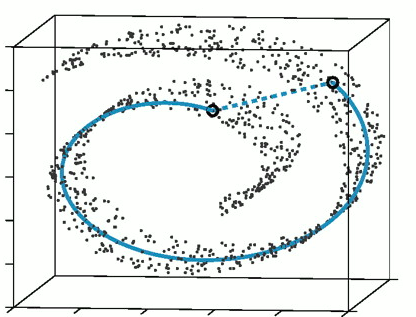
\includegraphics[width=3.5in]{./images/ISOMAP.png}
%label the figure so latex can reference it
\caption{For a linear method like PCA, the two circled points on the swiss roll would be close together even though they are far apart when using geodesic distances. Taken from \cite{TenenbaumJB2000Aggf}.}
      \label{fig:Swiss roll}
\end{figure}


\subsubsection{Multidimensional scaling (MDS)}
This idea of preserving relative distances between points in both the input space and embedded space is based on the multidimensional scaling (MDS) approach. Assume that an $n\times n$ matrix, $\Bm{B}$=(b$_{ij}$), of pair-wise distances (not necessarily Euclidean) or similarities (see appendix \ref{proximity}), $\Bm{S} = (s_{ij})$, between data points, $\{\vect{x}_{1}, \ldots, \vect{x}_{n} \}$, is given and $n$ is large.


MDS \cite{CoxT2000, MardiaK.V1979Ma} considers the the problem of finding a low dimensional model of the high dimensional data by searching for a configuration of $n$ points $\{\vect{y}_{1}, \ldots, \vect{y}_{n} \}$ in $\R^{\text{l}}, \text{l} \ll \text{n}$, where each $\vect{y}_{i}$ is a low dimensional representation of $\vect{x}_{i}$, and such that relative pair-wise distances between points are preserved. Specifically, the Euclidean distances between the configuration points, $\norm{\vect{y}_{i} - \vect{y}_{j}}_{2}$, must be as ``close" as possible to  the given distances, b$_{ij}$, that is, $\norm{\vect{y}_{i} - \vect{y}_{j}}_{2} \approx \text{b}_{ij}$, for all $1 \leq i, j \leq n$.

\subsubsection{Spectral non-linear dimensionality reduction}
Spectral non-linear dimensionality reduction (SNLDR) techniques are a 
class of MDS methods which find a low dimensional model of the data by preserving relative distances between neighboring points on a data manifold. These are the non-linear dimensionality reduction algorithms that we will consider. Examples of SNLDR methods include ISOMAP \cite{TenenbaumJB2000Aggf}, locally linear embedding (LLE)  \cite{roweis2000nonlinear}, Laplacian eigenmaps (LE) \cite{belkin2003laplacian} and diffusion maps \cite{coifman2006diffusion}, in addition to many others. Unlike linear dimensionality reduction techniques, SNLDR methods do not make apriori assumptions about the underlying geometry of the data manifold. SNLDR methods model local neighborhood relations between data points by building a graph on the data  \cite{Luxburg2007}. We only review the diffusion maps algorithm.


\subsubsection{Key graph theory concepts}
The non-linear dimensionality reduction algorithms we consider are based on graph theory. Hence, we first introduce three key graph theory concepts that we need: a weighted undirected graph, the degree matrix and the graph Laplacian.


A graph is a tuple $G = (V,E)$ where $V = \{v_1, \ldots , v_n\}$ is a finite set of points called vertices or nodes and $E$ is a finite collection of edges connecting pairs of vertices. The graph $G$, is undirected if the edges between vertices are bidirectional.
We can make a weighted graph by assigning a weight or number $w_{ij}$, to an edge $e_{ij} \in E$, between a pair of vertices $(v_i, v_j) \in V$. A connectivity matrix or similarity matrix $\Bm{W}$, of $G$, is the matrix whose $(i,j)$-th entries are edge weights $w_{ij}$.
The degree $d_i$, is the sum of weights $w_{ij}$, of all edges connected to a vertex $v_i \in V$.
A diagonal matrix $\Bm{D}$, with degrees, $d_{i}$, on its diagonal is called the degree matrix.
The unnormalized graph Laplacian is the  matrix $\Bm{L = D} - \Bm{W}$.


\subsubsection{Neighborhood graph}
We can approximate small distances between points in the input space using the usual Euclidean distance between nearby points in the embedded space as in linear approaches. However, long distances in the input space are not necessarily equal to long distances in the feature space (see figure \ref{fig:Swiss roll}). One way to address this problem is to ignore long distances in the embedded space by building a graph $G = (V, E)$ on the data. We ignore long distances by placing an edge $e_{ij} \in E$ only between neighboring vertices $(v_i, v_j) \in V$. The result is called 
a neighborhood graph.


A particular type of neighborhood graph is the $\epsilon-$neighborhood graph constructed as follows. Suppose we are given a data set, $\Bm{X} =  \{\vect{x}_{1}, \ldots, \vect{x}_{n} \}$ and assume that the pairwise distances, $b_{ij} = \text{dist}(\vect{x}_{i}, \vect{x}_{j})$, between points are known. Identifying each data point with a vertex $v_{i} \in V$, on a graph $G = (V, E)$, we can build a weighted  undirected graph on the data by placing an edge $e_{ij} \in E$, between vertices $(v_i, v_j) \in V$, if $x_i$ and $x_j$ are sufficiently close i.e., dist$(x_i, x_j) < \epsilon$. We weight the edge $e_{ij} \in E$, by a similarity measure $s_{ij}$, derived from the given distances (see appendix \ref{proximity}). The resulting $\epsilon-$nearest neighborhood graph represents the local distances among points.


For diffusion maps, the neighborhood graph is modified to a fully connected graph, but where the weights are approximately zero whenever the distance between data points is large.
To do this, we use a similarity function that captures local neighborhood relations between points and at the same time decays to zero so fast that we do not have to truncate the weights. In particular, in diffusion maps, we use the similarity function 
$$w_{ij} = \exp \{- \frac{\text{dist}^{2}(\vect{x}_i, \vect{x}_j)}{2 \sigma^2} \}.$$ 
In this way, $\sigma$ plays the role of $\epsilon$, in that it specifies the width of the neighborhood.

\subsubsection{Basic idea of the diffusion maps algorithm}
The diffusion maps algorithm consists of several steps which are outlined in appendix \ref{diffusion maps}. Below is a brief summary of the diffusion maps algorithm.

\begin{itemize}
\item[1)] Given the pairwise distance dist$(\vect{x}_i, \vect{x}_j)$, compute the weight matrix 
$\Bm{W} = (w_{ij})$, between data points by setting
$$w_{ij} = \displaystyle \exp \{- \frac{\text{dist}^{2}(\vect{x}_i, \vect{x}_j)}{2 \sigma^2} \}.$$
\item[2)] Let $d_{i} = \sum_{j = 1}^{n} w_{ij}$ be the degree of the $i^{th}$ node and compute the degree matrix $\Bm{D} = \text{diag}(d_{1}, \ldots, d_{n})$.
\item[3)] Define a random walk on the graph of the data (see appendix \ref{random walk}) by specifying $p_{ij} = \displaystyle \frac{w_{ij}}{d_{i}}$, the probability of going from vertex $v_i$ to $v_j$ in one-step. Organize the pair-wise transition probabilities in an $n \times n$ 
transition probability matrix $\Bm{P} = \Bm{D}^{-1}\Bm{W}$ with $\Bm{P} = (p_{ij})$.
\item[4)] Normalize $\Bm{P}$ to obtain a PSD similarity matrix $\Bm{S}$ given by
$\Bm{S} = \Bm{D}^{\frac{1}{2}}\Bm{P}\Bm{D}^{\frac{-1}{2}}$.
\item[5)] Compute the SVD of $\Bm{S}$ and write $\Bm{S} = \Bm{V}\bm{\Sigma}\bm{V^{\top}}$ where,
$\bm{\Sigma} = \text{diag}(\lambda_{0}, \ldots, \lambda_{n-1})$ with ordered eigenvalues, 
$\lambda_{0}\geq \lambda_{1} \geq \ldots \geq \lambda_{n-1}$ and corresponding eigen vectors 
$\Bm{V} = [v_0, v_1 \ldots, v_{n-1}]$.
\item[6)] The l-dimensional embedding of the $i^{th}$ data point $\vect{x}_i$
in the low dimensional space $\mathbb{R}^{l}$ is the map
$$ \vect{x}_{i} \mapsto  \begin{bmatrix}
         \lambda_{1}^{t}\phi_{1}(i)\\
         \lambda_{2}^{t}\phi_{2}(i)\\
         \vdots\\
         \lambda_{l}^{t}\phi_{l}(i)
        \end{bmatrix} .$$
where $\{ \phi_{0}, \phi_{1}, \ldots, \phi_{n-1} \}$ are the right singular vectors of $\Bm{P}$
and $\lambda_{i}^{t}$, are obtained from the t-step transition probability matrix $\Bm{P}^{t}$
(see appendix \ref{diffusion maps}).
\end{itemize}































%%%%%%%%%%%%%%%%%%%%%%%%%%%%%%%%%%%%%%%%%%%%%%%%%%%%%%%%%%%%%%%%%%%%%%%%%%%%%%%%%%%%%%%%%%%
%%%%%%%%%%%%%%Laplacian Eigen Maps algorithm %%%%%%%%%%%%%%%%%%%%%%%%%%%%%%%%%%%%%%%%%%%%%%
%\subsubsection{Laplacian eigen maps algorithm}
%Building a Graph from a data set $X = \{\vec{x}_{1}, \ldots , \vec{x}_{n}\}$}
%\pause
%Assuming the pairwise distances $d_{ij}$ or similarities $s_{ij}$ between data points $\{x_{1}, \ldots, x_{n}\}$
%are known, the points may be connected using 
%
%mutual k-nearest neighbor graph
%
%
%Build a weighted graph on the given data set
%by viewing data points as vertices of a graph in which neighboring points are connected by weighted edges
%
%From the adjacency matrix W  using one of the two methods
%
%Choose the weights $w_{ij}$ using the Heat Kernel with no parameter
%\[
% w_{ij} =
%  \begin{cases} 
%      \hfill e^{-\frac{\norm{\vec{x}_{i}-\vec{x}_{j}}^2}{t}}    \hfill & \text{ if $(i,j) \in E$} \\
%      \hfill 0 \hfill & \text{otherwise} \\
%  \end{cases}
%\]
%\pause
%
%\item Case 2: (No Parameter t).
%
%\[
% w_{ij} =
%  \begin{cases} 
%      \hfill 1    \hfill & \text{ if $(i,j) \in E$} \\
%      \hfill 0 \hfill & \text{otherwise} \\
%  \end{cases}
%\]
%
%
%
%
%
%and degree matrix D,
%compute the graph Laplacian L using the relationship L = D-W
%
%Solve the generalized eigenvalue problem Lv = $\lambda$Dv
%and stack the smallest  eigenvectors $\{\vec{v}_{1}, \ldots, \vec{v}_{d} \}$ of L excluding the smallest eigenevector of L as columns in a matrix U ;
%obtain a d-dimensional embedding of the data
% by viewing each  data point as the $i^{th}$ row of U via the map
%$\vec{x}_{i} \mapsto (\vec{v}_{1}(i), \ldots, \vec{v}_{d}(i))$ };
%
%
%
%
%
%
%\item Solve the generalized eigenvalue problem $L\vect{v} = \lambda D \vect{v}$ and take the bottom d-smallest generalized eigenvectors $\vect{f}_{2}, \ldots, \vect{f}_{d}$ of L excluding the constant eigenvector.
% \pause
% \item Form the matrix U = $[\vect{f}_{2} \ldots \vect{f}_{d}]$ by stacking $\vect{f}_{i}$ as columns in U.
% \pause 
% \item View the $\text{i}^{th}$ row of U as the $d$-dimensional representation of the $\text{i}^{th}$ vertex 
% corresponding to the original data point $\vect{x}_{i}.$
%




























